\section{Internal implementation}

\subsection{Overall architecture}

\begin{figure}[H]
    \centering
    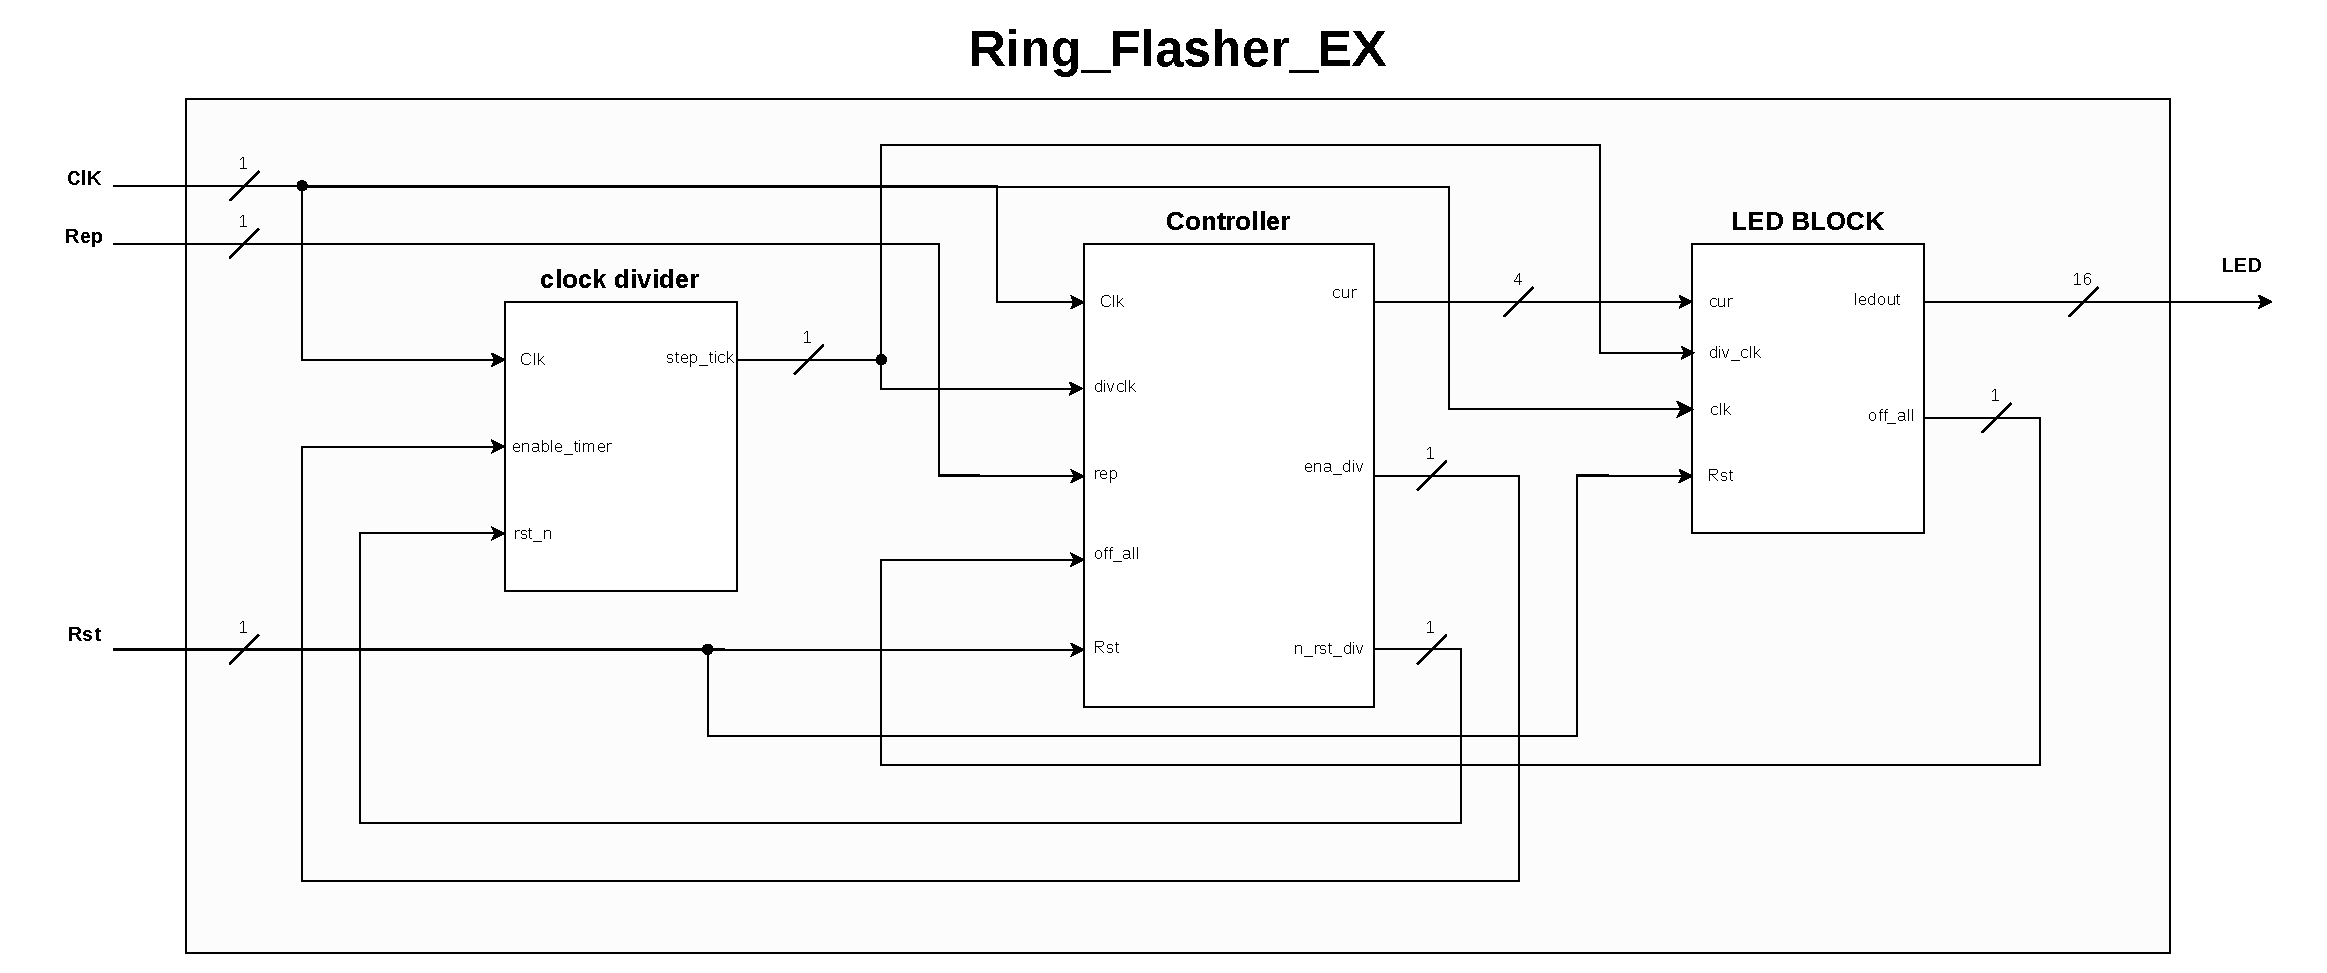
\includegraphics[width=1\linewidth]{graphics/Internal_lab1.pdf}
    \caption{The Block diagram of the Ring Flasher module.}
\end{figure}

\subsection*{Table 1: Top-Level Module (Ring\_Flasher\_EX)}
\begin{tabular}{lp{2.5cm}llp{6cm}}
\toprule
\textbf{Component} & \textbf{Signal Name} & \textbf{Direction} & \textbf{Width} & \textbf{Description} \\
\midrule
External Interface & clk  & Input  & 1-bit  & Main system clock source. \\
                  & rep  & Input  & 1-bit  & Repeat control signal for sequence logic. \\
                  & rst  & Input  & 1-bit  & Global system reset. \\
                  & LED  & Output & 16-bit & Final output bus driving the hardware LEDs. \\
\midrule
Clock Divider      & step\_tick     & Output & 1-bit & Pulse used to update the sequence timing. \\
                  & enable\_timer  & Input  & 1-bit & Control signal to activate the internal timer. \\
                  & rst\_n         & Input  & 1-bit & Active-low reset for the divider sub-module. \\
\midrule
Controller         & cur        & Output & 4-bit & Current LED index for the sequence. \\
                  & ena\_div    & Output & 1-bit & Enable signal sent to the clock divider. \\
                  & n\_rst\_div & Output & 1-bit & Dedicated reset for the internal divider logic. \\
                  & off\_all    & Input  & 1-bit & Feedback signal indicating all LEDs are off. \\
\midrule
LED BLOCK          & ledout     & Output & 16-bit & Internal LED drive bus. \\
                  & off\_all    & Output & 1-bit  & NOR-reduction output used to detect when all LEDs are off. \\
\bottomrule
\end{tabular}

\vspace{1cm}

\begin{figure}[H]
    \centering
    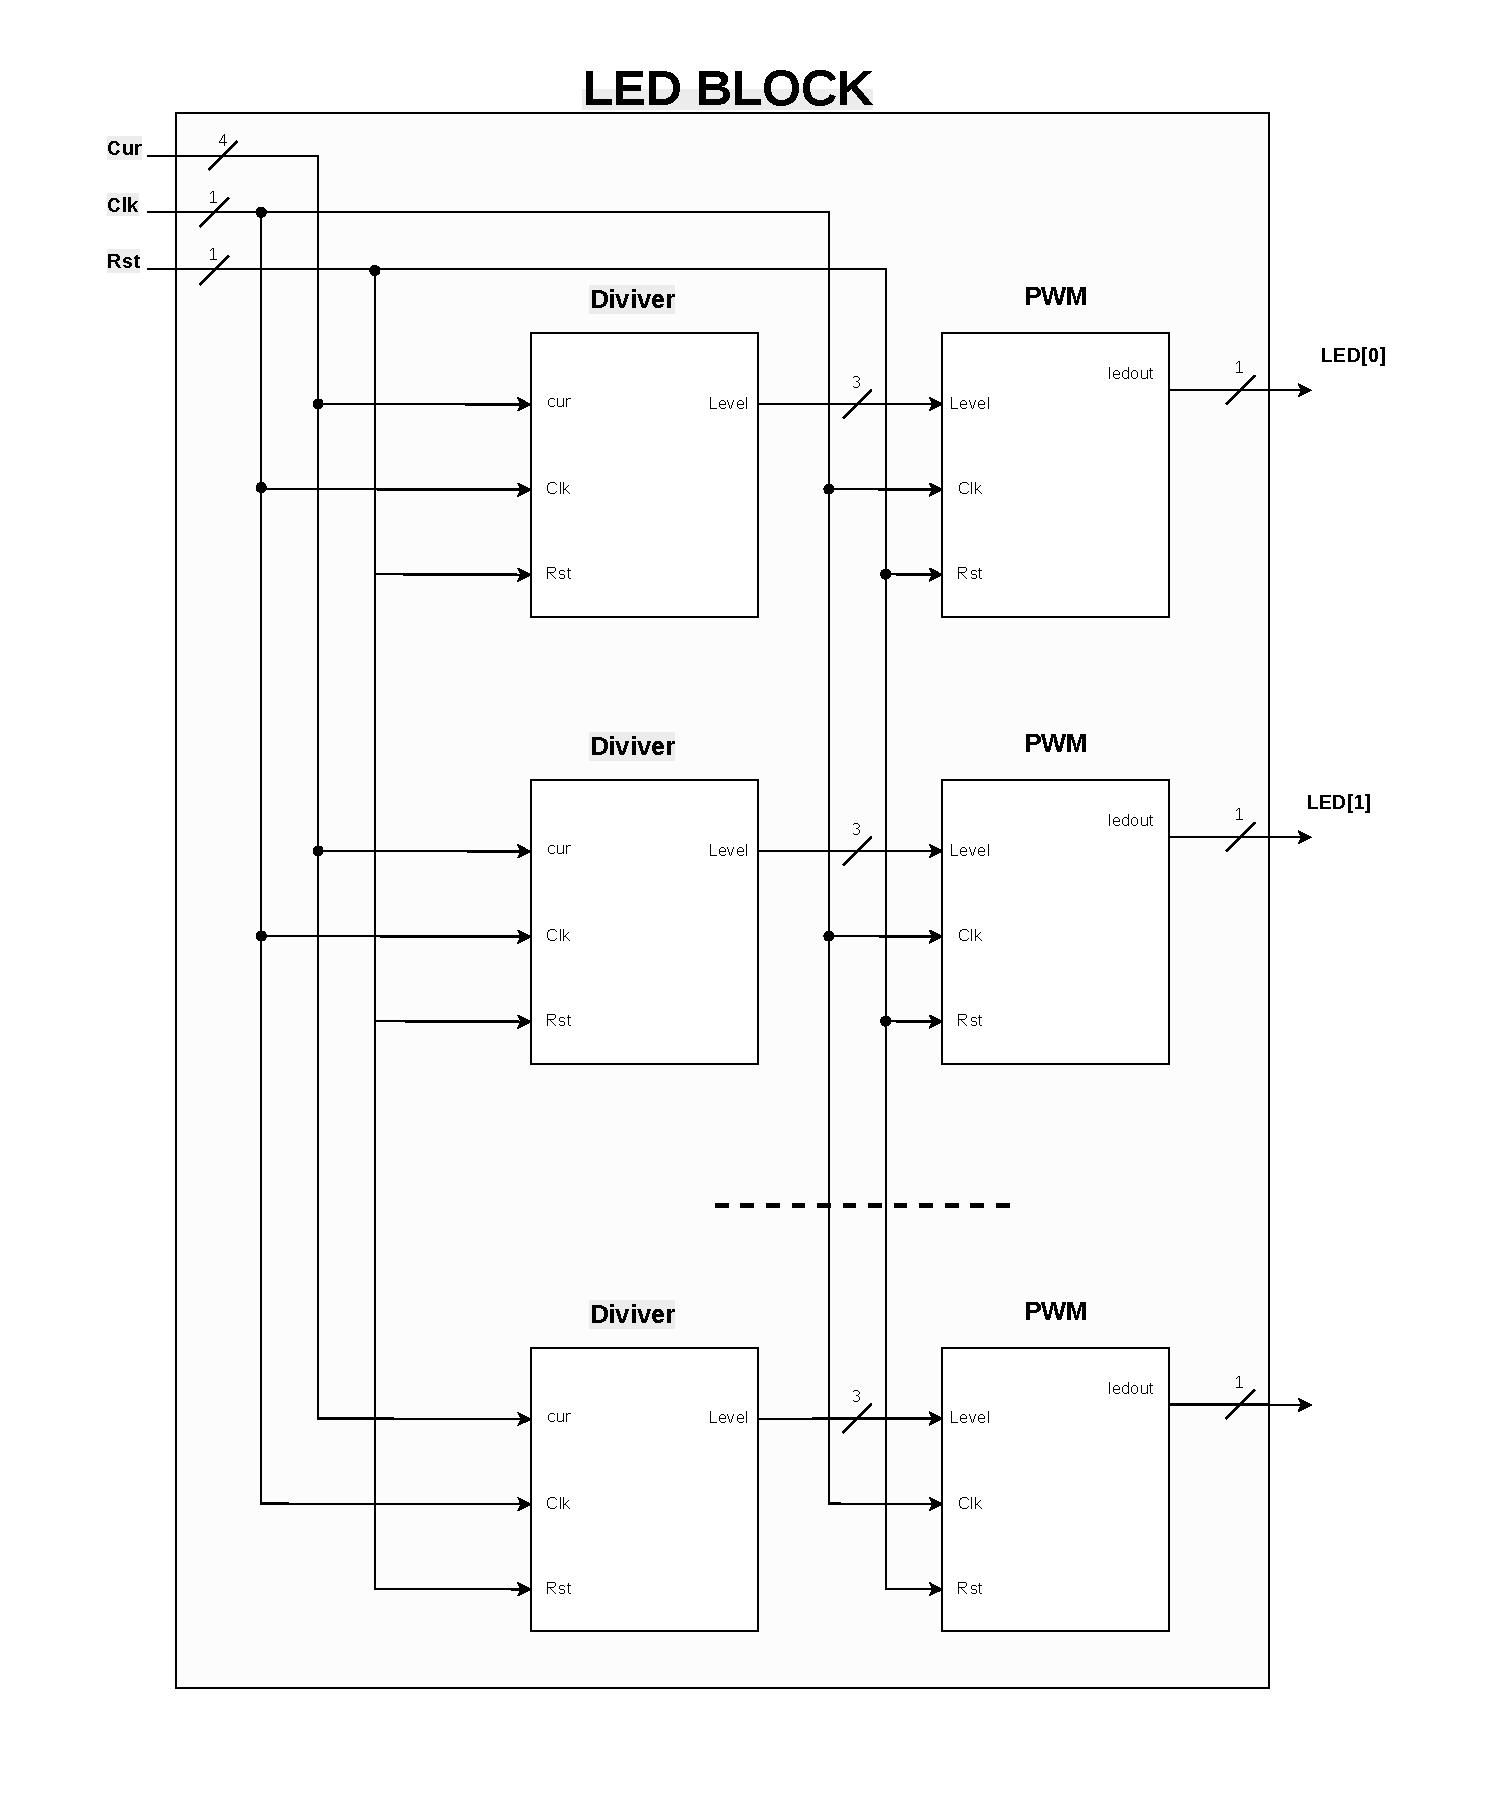
\includegraphics[width=1\linewidth]{graphics/Internal_lab1.1.pdf}
    \caption{The Block diagram of the LED BLOCK.}
\end{figure}

\subsection*{Table 2: LED BLOCK Internal Structure}
\renewcommand{\arraystretch}{1.2}
\begin{tabular}{>{\raggedright\arraybackslash}p{2.6cm} p{2.4cm} l l p{6cm}}
\toprule
\textbf{Sub-Module} & \textbf{Signal Name} & \textbf{Direction} & \textbf{Width} & \textbf{Description} \\
\midrule
\multirow{3}{*}{LedStatus} & cur    & Input  & 4-bit & Current LED position from the Controller. \\
                           & led\_id & Input  & 4-bit & Index of the LED block being controlled. \\
                           & level   & Output & 3-bit & Brightness level of the corresponding LED. \\
\midrule
\multirow{4}{*}{PWM}       & clk     & Input  & 1-bit & System clock used for PWM generation. \\
                           & reset   & Input  & 1-bit & Reset signal for the PWM logic. \\
                           & level   & Input  & 3-bit & Brightness level received from LedStatus. \\
                           & ledout  & Output & 1-bit & PWM output that drives one LED channel. \\
\midrule
NOR Reduction Gate         & input   & Input  & 16-bit & LED brightness vector used to detect when all LEDs are off. \\
                           & off\_all & Output & 1-bit & Goes high when all LED brightness levels are zero. \\
\bottomrule
\end{tabular}
\subsection{State machine}

\begin{figure}[H]
	\centering
	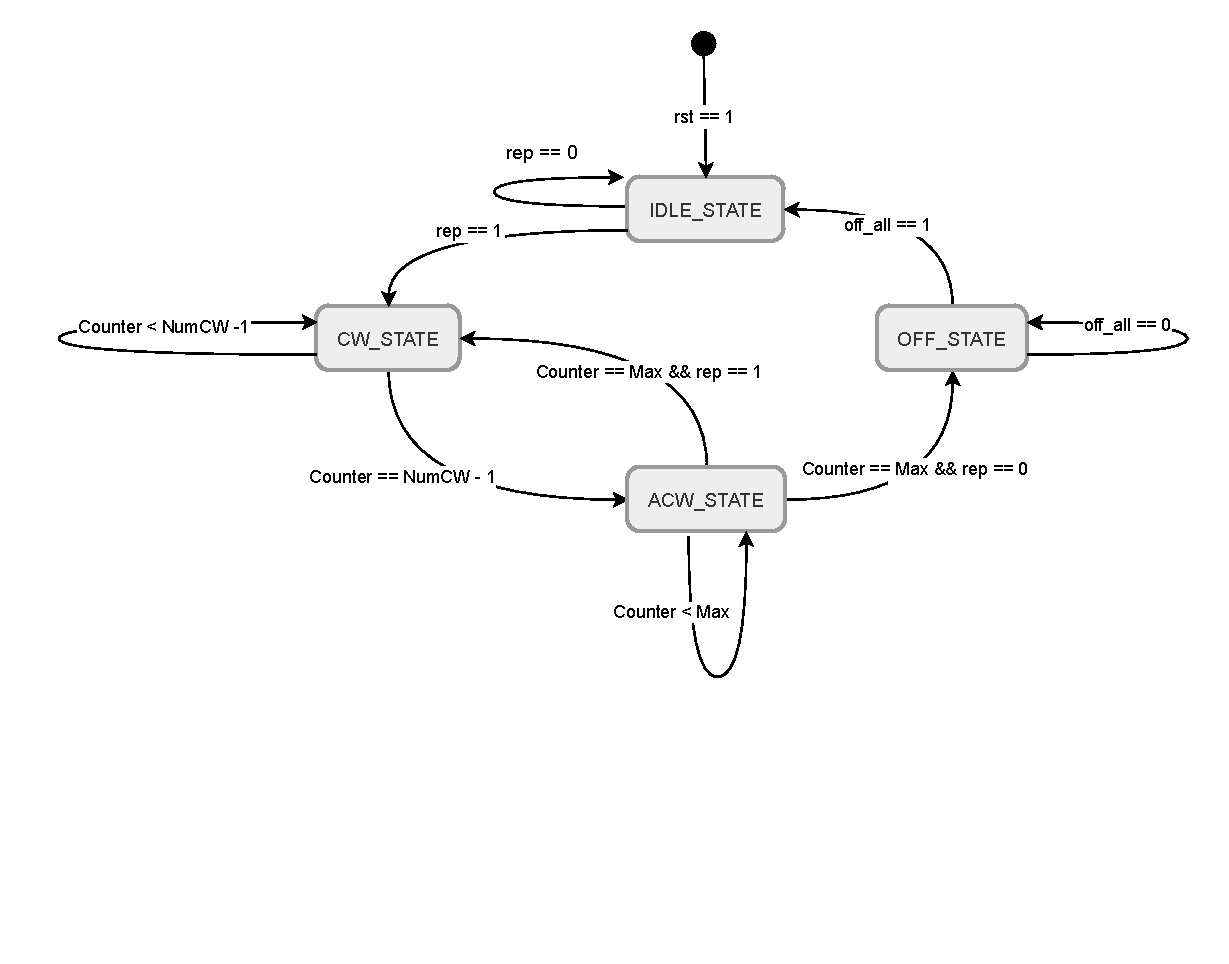
\includegraphics[width=1\linewidth]{graphics/FSM_lab1.pdf}
	\caption{Finite state machine of the Ring Flasher module.}
	\label{fig:fsm_ring_flasher}
\end{figure}

\noindent\textbf{Parameters}
The finite state machine is implemented in the \texttt{Control} module with the following parameters:
\begin{itemize}
	\item \texttt{NumLed = 16}: number of LEDs in the ring.
	\item \texttt{NumCW = 12}: number of clockwise (CW) steps.
	\item \texttt{NumACW = 8}: number of anti-clockwise (ACW) steps.
	\item \texttt{IDLE\_STATE = 0}: idle state.
	\item \texttt{CW\_STATE = 1}: clockwise motion state.
	\item \texttt{ACW\_STATE = 2}: anti-clockwise motion state.
	\item \texttt{OFF\_STATE = 3}: turn-off state until all LEDs fade out.
\end{itemize}

\noindent\textbf{Variables}
\begin{itemize}
	\item Inputs: \texttt{clk}, \texttt{divclk}, \texttt{rep}, \texttt{rst}, \texttt{off\_all}.
	\item Outputs: \texttt{cur}, \texttt{ena\_div}, \texttt{n\_rst\_div}.
	\item State registers: \texttt{State}, \texttt{NextState}.
	\item Counters: \texttt{Counter}, \texttt{NextCounter}.
	\item LED position registers: \texttt{cur\_pos}, \texttt{next\_pos}.
\end{itemize}



\subsection*{Table 4: Variable Name of State Machine}
\renewcommand{\arraystretch}{1.2}
\begin{tabular}{p{2.6cm} p{2.2cm} p{3.6cm} p{6.0cm}}
\toprule
\textbf{Variable Name} & \textbf{Type} & \textbf{Width} & \textbf{Description} \\
\midrule
\texttt{State} & Reg & 2-bit & Current FSM state register. \\
\texttt{NextState} & Reg & 2-bit & Next-state combinational register. \\
\texttt{Counter} & Reg & $\log_2(NumCW+NumACW)$ + 1 & Counts total steps in CW and ACW phases. \\
\texttt{NextCounter} & Reg & $\log_2(NumCW+NumACW)$ + 1 & Next value of step counter. \\
\texttt{cur\_pos} & Reg & $\log_2(NumLed)$ + 1 & Current LED pointer position. \\
\texttt{next\_pos} & Reg & $\log_2(NumLed)$ + 1 & Next LED pointer position. \\
\texttt{cur} & Wire (output) & $\log_2(NumLed)$ + 1 & Exported LED index to datapath. \\
\texttt{ena\_div} & Reg (output) & 1-bit & Enable signal for clock divider. \\
\texttt{n\_rst\_div} & Reg (output) & 1-bit & Active-low reset signal for divider. \\
\bottomrule
\end{tabular}
\\
The signal \texttt{cur} provides the current LED index to the datapath. The control outputs \texttt{ena\_div} and \texttt{n\_rst\_div} are used to enable and reset the step-timer clock divider.

\noindent\textbf{State-by-State Behavior}
\begin{itemize}
	\item \textbf{IDLE\_STATE}: The system waits for \texttt{rep = 1}. If \texttt{rep = 0}, the divider is disabled and held in reset. When \texttt{rep = 1}, the FSM moves to \texttt{CW\_STATE}, initializes \texttt{Counter = 0}, and starts from position \texttt{0}.

	\item \textbf{CW\_STATE}: At each \texttt{divclk} tick, the position moves clockwise and \texttt{Counter} is incremented. When \texttt{Counter = NumCW - 1}, the FSM transitions to \texttt{ACW\_STATE}.

	\item \textbf{ACW\_STATE}: At each \texttt{divclk} tick, the position moves anti-clockwise and \texttt{Counter} is incremented. When \texttt{Counter = NumCW + NumACW - 1}, the FSM checks \texttt{rep}: if \texttt{rep = 1}, it returns to \texttt{CW\_STATE} with \texttt{Counter = 0}; otherwise, it enters \texttt{OFF\_STATE}.

	\item \textbf{OFF\_STATE}: No new LED position is injected (position is forced to an invalid index). The datapath keeps decreasing LED intensity until all LEDs are off. When \texttt{off\_all = 1}, the FSM returns to \texttt{IDLE\_STATE}.
\end{itemize}

\subsection*{Table 3: State Name of State Machine}
\renewcommand{\arraystretch}{1.2}
\begin{tabular}{lll p{8cm}}
\toprule
\textbf{State Name} & \textbf{Parameter} & \textbf{Code} & \textbf{Description} \\
\midrule
IDLE & \texttt{IDLE\_STATE} & 2'd0 & Wait state. The FSM stays here until \texttt{rep = 1}. \\
CW & \texttt{CW\_STATE} & 2'd1 & Clockwise running state. LED position increments each step. \\
ACW & \texttt{ACW\_STATE} & 2'd2 & Anti-clockwise running state. LED position decrements each step. \\
OFF & \texttt{OFF\_STATE} & 2'd3 & Fade-out state. Waits until all LEDs are fully off before returning to IDLE. \\
\bottomrule
\end{tabular}
